

\newpage
\section{Design and Implementation} \ref{sec:dai}
This section will be discussing the main contribution of this project: a implementation of lattice Boltzmann method on SpiNNaker.  \\

All the source code is available at: \url{https://github.com/YuaNFrank/SpiNN_LB}.
\subsection{Implementation Overview}

As we discussed at \ref{sec:sdw}, in general SpiNNaker development workflow, the first thing we did is to define the computation graph in Python. We will discuss how we define the lattice vertex (\ref{sec:tlc}), how we define our edge (\ref{sec:tle}), and how we connect them together as a graph (\ref{sec:tcg}). All these steps are implemented in Python API.
1       
Then on the computation side, as discussed at \ref{sec:lbmb}, there are five step for a lattice Boltzmann method in general. While the first four steps do not involve communication, and can be calculate locally for each lattice vertex (discussed at \ref{sec:cp}), the last step, the streaming step, is where the communication happens, which we will focus on at \ref{sec:ssc}. These computation-wise code is written in C.

\subsection{The Lattice Cell} \label{sec:tlc}
\subsubsection{Design Consideration} \label{sec:tlcdc}
In the lattice cell class, we will define the data regions needed for simulation. In implementation, it need to acquire those data, reserve memory for the data and pass the data in SpiNNaker SDRAM in Python, then define how to read the data from the SDRAM during simulation in C. The data regions that a lattice might need for simulation are: \\

\begin{itemize}
    \item \textbf{System Information:} for every simulation, they at least need some memory reserved for the runtime system such as the how long is a machine time step. And the developers need to generate the system data region and allocate memory for them manually.
    
    \item \textbf{Transmission Information:} for non-embarrassingly parallel problems, the simulation are involved in communication. The keys are generated by the runtime, and the developers can ask the runtime for a fix number of keys for every lattice. The developers need to allocate memory for the transmission keys and pass the keys to the cores, correspondingly.

    \item \textbf{Position Information:} in lattice Boltzmann, a lattice might need to know what is its position \textbf{(x,y)} among the whole simulation lattices. The position information would be generated when connecting the lattices as a graph, and then pass them into the application.
    
    \item \textbf{Initialized Velocity:} in lattice Boltzmann method, the velocity need to be generated according to the specific problem. We can either initialize it in Python then pass then in or initialize it in the simulation according to the position. A more detailed discussion is at \ref{sec:ip}.
    
    \item \textbf{Routing Information of Neighbours:} in lattice Boltzmann method, the lattice need to exchange the momentum and energy by moving the distribution function with its eight neighbours. This involve a few communication and the lattice need to know which are its eight neighbours and their routing information i.e. routing keys to communicate with them. Thus allocating memory and pass them into the cores is necessary. 
    
    \item \textbf{Index of this Lattice:} we might need to know the index of the lattice in the whole simulation fabric. This might not be necessary for a simple prototype. Since the random number generation is relatively slow, we can use it as a random number in practice. A further discuss is at \ref{sec:ssc}.
    
    \item \textbf{Result Recording:} the SDRAM in SpiNNaker is relatively limited (\ref{sec:sa}). We can use the recorded data to store larger simulation result more reliably. We can specify the an area of memory used for recording the results and get them back when the simulation ends.
\end{itemize}

\subsubsection{Final Implementation}
In the final implementation, we defined the discussed data regions in the \textit{LatticeBasicCell} class following the pattern: get the data; allocate memory; write the data in. For different data, there are different way to get the data:

\begin{itemize}
    \item \textbf{System Information:} the \textit{SpiNNaker GraphFrontEnd} provide API to generate the system data region.
    \item \textbf{Transmission Information:} the SpiNNaker runtime would allocate keys for the cores.
    \item \textbf{Position Information:} the position information is decided during runtime. it will be passed as class variables.
    \item \textbf{Initialized Velocity:} the velocities are decided during runtime with a initialization function. They will be passed as class variables. 
    \item \textbf{Routing Information of Neighbours:} a lattice can know the which are its neighbours by asking the connected edges. We will illustrate how we implement it at \ref{sec:tle}. After knowing its neighbours, we can get their routing keys via the get\_routing\_info\_from\_pre\_vertex() function from the \textbf{PACMAN} library.
    \item \textbf{Index of Lattice:} we can ask the graph system for the index of a lattice.
    \item \textbf{Result Recording:} we do not need to get data from result recording since it is for the result.
\end{itemize}

After all the data are acquired, we get then reserve corresponding memory and write the data into the SDRAM of each SpiNNaker core; see the upper part of Fig.~\ref{fig:write_data}. Correspondingly, in the C file, we also need to read the data from the SDRAM before the simulation; see the bottom part of Fig.\ref{fig:write_data}. The Fig.~\ref{fig:write_data} shows how we reserve memory for the different data regions and write the data into the SDRAM followed by how to read the written data from the SDRAM during runtime in C.
\begin{figure}[tb]
   \centering
       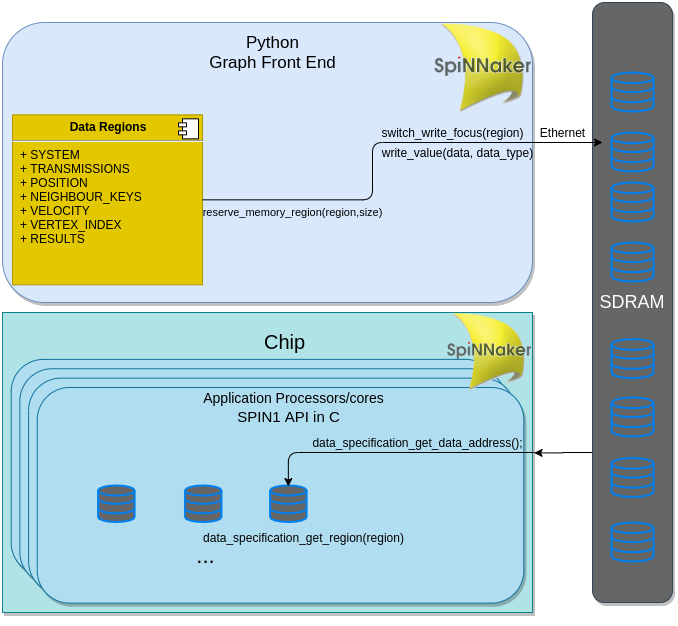
\includegraphics[width=1\textwidth]{figures/write_data.png}
       \caption{A lattice cell A connected by another lattice B via a lattice edge with the compass being "W". The lattice A then can get the routing key from its pre\_vertex, B.}
       \label{fig:write_data}
\end{figure}



\subsection{The Lattice Edge} \label{sec:tle}
\subsubsection{Design Consideration}
The major job of the lattice edge except connecting two lattice cells is providing a way that the lattice cell can get the vertex on the other end of this edge in a given direction. So that each lattice can get the routing information (routing keys) of its eight neighbours with knowing the direction. 
\subsubsection{Final Implementation}
In the implementation, the \textit{Lattice Edge class} inherit from the \textit{MachineEdge}, which provided a way to record the pre-vertex and post-vertex, from the \textbf{PACMAN} library. Then we introduced another attribute, \textbf{compass}, to record the relative position of the pre-vertex; see Fig.~\ref{fig:edge}.
\begin{figure}[tb]
   \centering
       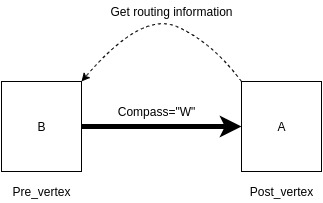
\includegraphics[width=0.7\textwidth]{figures/edge.jpg}
       \caption{A lattice cell A connected by another lattice B via a lattice edge with the compass being "W". The lattice A then can get the routing key from its pre\_vertex, B.}
       \label{fig:edge}
\end{figure}

\subsection{The Computational Graph} \label{sec:tcg} 
\subsubsection{Design Consideration}
In the selected test problem from Minion and Brown\cite{minion1997performance}, the boundary condition we applied for this project is a periodic condition. In the C implementation, we implemented the periodic condition is halo-swapping; see Fig.~\ref{fig:haloswap}. The periodic condition is explicitly applied to the post-collision distribution function $f_i^{*}$ in the streaming step, which introduced extra memory consumption and complexity into the development.

Fortunately, in SpiNNaker, the developers do not implement the halo-swapping to apply to the periodic condition explicitly. Instead, SpiNNaker developers can simply connect the lattices on one fringe to the lattices on the opposite fringe via the implemented \textit{Lattice Edge}; see Fig.~\ref{fig:spinnaker_halo}.


\begin{figure}[!tb]

\begin{subfigure}[b]{1\textwidth}
       \centering
       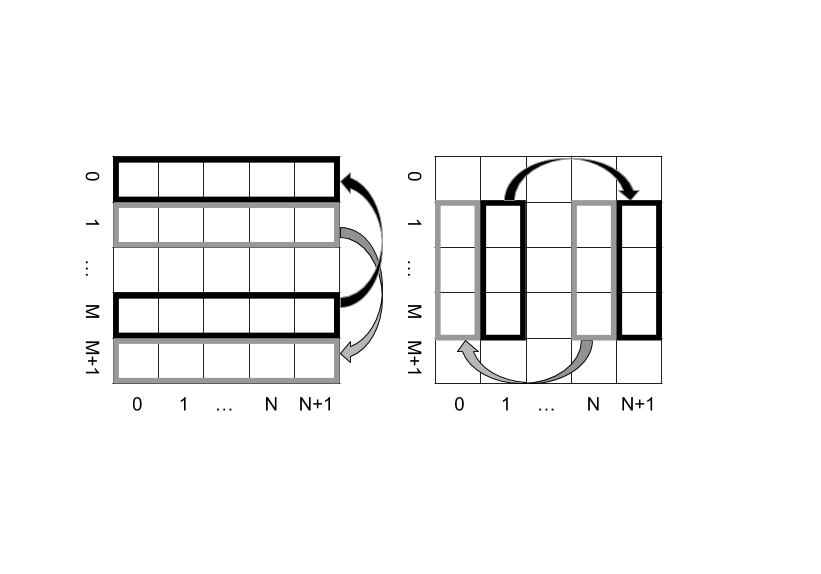
\includegraphics[width=0.8\textwidth]{figures/haloswap.png}
       \caption{A periodic condition in M$\times$N lattice Boltzmann implemented by halo-swapping. We apply this method in our serial C implementation.}
       \label{fig:haloswap}
   \end{subfigure}
   \begin{subfigure}[b]{1\textwidth}
       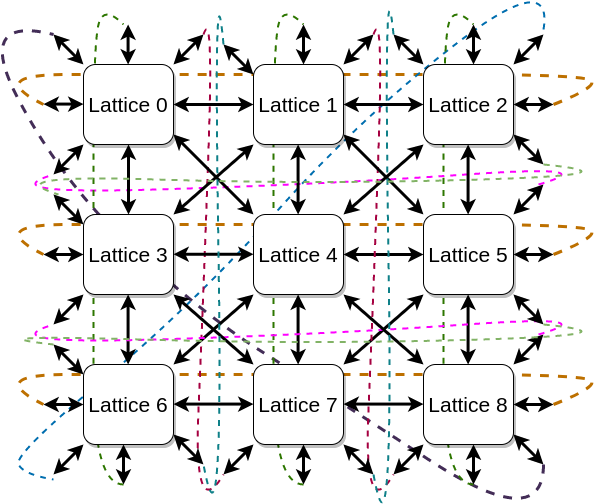
\includegraphics[width=\textwidth]{figures/2dfabric.png}
       \caption{A periodic condition in 3$\times$3 lattice Boltzmann implemented by connecting the lattice periodically via lattice edge. We apply this method in the SpiNNaker implementation.}
       \label{fig:spinnaker_halo}
   \end{subfigure}
\end{figure}

\subsubsection{Final Implementation}
As we designed, to implement a periodic condition, we connect the lattice cells periodically via lattice edge; see Algo.~\ref{algo:periodic}.

\begin{algorithm}
 \caption{The Algorithm to connect the lattice with a periodic condition}
 \label{algo:periodic}
 \KwData{Scale in x dimension: X; Scale in y dimension: Y}
 \For{i in 0...X}{
    \For {j in 0...Y} {
       
    }
 }

\end{algorithm}




\subsection{Initialize Parameters} \label{sec:ip}
\subsubsection{Design Consideration}
To initialize the parameters for the lattice Boltzmann, there are two different ways in general. The first one is initialization on host (in Python) then passing the initialized parameters into the simulation, and the other one is initialization on SpiNNaker (in C).\\

When initializing parameters in Python on host, we need to compute the parameters in serial nested loops before the SpiNNaker actually run the simulation. On contrast. If we initializing the parameters in SpiNNaker, the parameters would be computed distributively on each individual core. Beside, vanilla Python is commonly regard as being poor in scientific computing, especially in nested loop.\\

It is obvious that initialization in C on the simulation runtime would be faster in speed comparing with initialization in Python in serial. Thus, our first implementation was based on C and compute the initial parameters distributively on each core. \\

However, there are two points in SpiNNaker that we do not take into consideration. The first one is that, as we introduced before, SpiNNaker is using ARM968 cores which have no floating point hardware and we have to use fixed-point arithmetic or a software-based floating-point arithmetic. It introduced some challenges in using mathematical library in C including \textbf{math.h}. The other one is that, as we also introduced before, the SpiNNaker cores have relatively limited ITCM (instruction tight-coupled memory). If we are plan to use mathematical library such as \textbf{math.h}, the library would run out of the limited ITCM. Although it is possible to implement mathematics functions such as \textbf{tanh} by applying the Taylor series, the accuracy and efficiency of the hand-write functions do not satisfy the requirements of this simulation.\\

After carefully reconsider the whole process, we finally decided to implement the initialization on the host in Python and then pass the initialized parameters as data regions to the SpiNNaker device.
\subsubsection{Final Implementation}


\subsection{Computation Implementation} \label{sec:cp}
\subsubsection{Design Consideration}
\subsubsection{Final Implementation}

\subsection{Streaming Step -- Communication Implementation} \label{sec:ssc}
\subsubsection{Design Consideration}
\subsubsection{Implementation}

\subsection{Communication Optimization}
\subsubsection{Design Consideration}
\subsubsection{Final Implementation}